\documentclass{article}
\usepackage[margin=1in]{geometry}
\usepackage[utf8]{inputenc}
\usepackage{amsmath}
\usepackage[hyphens]{url}
\usepackage{hyperref}
\usepackage[usenames,svgnames,dvipsnames]{xcolor}
\usepackage[pdftex]{graphicx}
\hypersetup{
	colorlinks=true,
    citecolor=DarkGreen,
    linkcolor=NavyBlue,
    urlcolor=blue,
    filecolor=green,
    bookmarksopen=true
}
\begin{document}

\title{Uma análise da naturalidade de síntese de fala com redes neurais no português em cenários de restrição}

\maketitle

\section{Introdução}
O texto apresentado nessa seção é um adendo ao texto principal com intuito de tratar objetivamente dos objetivos da pesquisa e da metodologia planejada. As seções aqui citadas farão referência ao texto principal visando facilitar a futura junção dos textos.
\subsection{Contextualização}
%Seção onde é feita a introdução da observação feita
A fala é o meio mais comum de comunicação entre seres humanos\cite{flanang}. 
A expressão falada é um dos meios que trocamos cotidianamente ideias, emoções e refletimos nossas personalidades\cite{Tiwari2012}. 
Computadores têm se tornado cada vez melhores na complexa tarefa que é interagir conosco usando a fala \cite{HCI-voice} tanta na tarefa de compreensão (\emph{Speech to Text} (STT)) quanto na síntese (\emph{Text to Speech} (TTS)). 

A síntese de fala já é um problema com vários produtos disponíveis para uso pelo público \footnote{\url{https://cloud.google.com/text-to-speech/}}\footnote{\url{https://azure.microsoft.com/en-us/services/cognitive-services/text-to-speech/}} presente no cotidiano de muitos através das mais diversas aplicações.
Entretanto esses modelos costumam permitir apenas síntese de falantes pré-determinados e frequentemente são modelos pagos e proprietários. 
Recentemente diversas pesquisas demonstraram excelentes resultados na criação de modelos de voz , seja o processo completo de síntese ou parte, a partir de gravações de um ou mais falantes na língua inglesa com modelos neurais.
Podemos destacar a grande influência dos trabalhos do Baidu com o Deep Voice\cite{deepVoice,deepVoice2,deepvoice3, baiduVoiceClonning} e da Google com o Tacotron \cite{tacotron,tacotron2, wavenet} todos com propostas similares de módulos neurais.

\subsection{Questão de Pesquisa e Hipóteses}
\label{sec:hipoteses}
%Seção onde as questões são introduzidas
Será que podemos obter a síntese de fala com esses modelos na língua portuguesa para um falante qualquer com resultados similares?
Essa mesma síntese pode ser obtida com resultados satisfatórios com restrições de tempo e de dados em seu treinamento?
Como podemos medir de maneira quantitativa os resultados de modelos de síntese de modo a facilitar a avaliação qualitativa?

%Seção onde destrinchamos as questões em hipóteses
Para validar essas questões devemos responder várias hipóteses como:

\begin{enumerate}
	\item \label{it:h1} Podemos treinar os mesmo modelos com dados em português?
	\item \label{it:h2} Podemos medir esses modelos treinados de maneira similar a proposta nos trabalhos?
	\item \label{it:h3} Podemos aproveitar algum conhecimento aprendido de outro conjunto de dados no nosso treinamento? 
	\item \label{it:h4} Podemos reduzir o conjunto de dados disponíveis e obter resultados comparavelmente bons?
	\item \label{it:h5} Podemos restringir o tempo de treinamento do modelo e obter resultados comparavelmente bons?
\end{enumerate}

Queremos levantar comparativamente se um modelo pré-treinado em outra língua que já tenha apresentado bons resultados perceptuais pode ser benéfico para a síntese na língua portuguesa observando-se o tempo de treinamento, a convergência da função de erro do modelo e a avaliação perceptual de um grupo de ouvintes.
Para responder essas questões estabelecemos uma sequência de decisões e experimentos destrinchados na próxima sessão.

\section{Metodologia}

Queremos levantar como os atuais algoritmos de síntese neural se comportam perceptualmente na língua portuguesa com restrições de dados e de tempo na geração do modelo. 
A primeira decisão é a escolha do modelo neural a qual desejamos replicar. 
Por uma questão de custo de implementação decidi abordar apenas um modelo, o Tacotron 2 \cite{tacotron2} desenvolvido pela Google cuja implementação encontra-se disponível em código aberto\footnote{\url{https://github.com/carpedm20/multi-speaker-tacotron-tensorflow}}.
O modelo também foi escolhido pois apresentar os melhores resultados de acordo com o comparativo levantado de modelos de síntese no inglês em Dezembro de 2017\footnote{\url{https://paperswithcode.com/sota/speech-synthesis-on-north-american-english}}.
Tendo sido fixado o modelo a ser utilizado estabelecemos também conjuntos de dados a serem utilizados nessa atividade como pode ser visto na Tabela \ref{tab:datasets}.

\begin{center}
	\begin{table}[h!]
		\begin{tabular}{p{1cm}p{2cm}p{5cm}p{6cm}}
			\hline
			Sigla & Nome              & Tópico& Descrição Técnica\\ 
			\hline
			\hypertarget{CONST}{CONST} & Constituição      & Leitura da constituição nacional cujo texto e arquivos de áudio original foram processados pela equipe FalaBrasil de modo a adequar-se às necessidades do estudo de fala                          & Segmentados em aproximadamente 30 segundos, falante masculino, em ambiente de gravação de rádio. 9000 arquivos; aproximadamente 9h de gravações\\
			\hline
			\hypertarget{LAPS}{LAPS}  & LAPS BenchMark    & Corpus de voz utilizado para avaliação de desempenho de sistemas LVCSR.& 700 frases, o corpus possui 35 locutores com 20 frases cada, sendo 25 homens e 10 mulheres, o que corresponde a aproximadamente 54 minutos de áudio\\ 
			\hline
			\hypertarget{YT}{YT}    & Youtube (Cellbit) & Áudios extraídos de vídeos do YouTube de um \textit{youtuber} no estilo \textit{vlog}. Legendas manualmente inseridas nos vídeos pelo próprio autor dos vídeos. & 23 vídeos com legenda publicados entre 04/07/2017 e 27/03/2018 totalizando aproximadamente 23h de áudio. O locutor é um youtuber do sexo masculino com 21 anos. Os arquivos foram seccionados baseado nos tempos de cada linha inteira do arquivo de legenda. 4203 arquivos (2.9$\pm$4.2s). \\ 
			\hline
		\end{tabular}
		\caption{Descrição dos Datasets}
		\label{tab:datasets}
	\end{table}
\end{center}

Esses dados foram selecionados fruto de uma pesquisa de dados anotados em português com amostras de falantes e frases.
Os dados \hyperlink{CONST}{CONST} e \hyperlink{LAPS}{LAPS} foram obtidos através do projeto FalaBrasil \cite{falabrasil}.
Originalmente os dados de \hyperlink{CONST}{CONST} foram obtidos da Câmara dos Deputados\footnote{\url{http://bd.camara.gov.br/bd/handle/bdcamara/1708}} mas como foram posteriormente anotados, alinhados e seccionados por frase mantemos a referência do grupo FalaBrasil.
Os dados \hyperlink{YT}{YT} foram obtidos de um canal do YouTube especificado na tabela com o intuito de fornecer uma fonte de áudio menos estruturada, menos formal e de fácil acesso público permitindo a qualquer um replicar o experimento com outro falante e uma estratégia comparativa similar.

Fazendo um mapeamento direto com os questionamentos levantados em \ref{sec:hipoteses} propomos os experimentos e avaliações abaixo.
Cada tópico está propondo alguma solução para o problema levantado na questão respectiva. 
\begin{enumerate}
	\item Os dados apresentados possuem formato similar ao utilizado no modelo pré-treinado de referência. 
	Sendo assim com pequenos ajustes pode ser facilmente adaptado para responder o questionamento \ref{it:h1}
	\item Para estabelecer-se uma linha de comparação treinaremos um modelo para cada conjunto de dados apresentado com 100\% dos dados de cada.
	Uma primeira métrica proposta a ser avaliada para responder ao questionamento \ref{it:h2} é o MOS Score que consiste na média de opiniões coletadas de ouvintes que avaliaram a síntese do modelo perceptualmente.
	Essa métrica é utilizada no trabalho escolhido e facilitará a comparação de resultados
	\item Para responder ao questionamento \ref{it:h3} podemos nos utilizar de \textit{transfer learning}\footnote{\url{https://machinelearningmastery.com/transfer-learning-for-deep-learning/}} com um modelo pré-treinado no inglês.
	O intuito de se aproveitar do \textit{transfer learning} é observar se as características aprendidas pelo modelo em uma língua podem ser aproveitadas em outra
	% pode haver correlação direta dada a natureza similar de sintaxe e semântica de ambas as línguas. Seja na ordem da construção das frases, nas raízes linguísticas  Auroux, Sylvain (2000). History of the Language Sciences. Berlin, New York: Walter de Gruyter. 1156 páginas. ISBN 3110167352
	\item Para responder o questionamento \ref{it:h4} propomos utilizar frações (5, 15, 33 e 50\%) dos dados apresentados para comparar seus resultados com o modelo base treinado com 100\% dos dados
	\item Para responder o questionamento \ref{it:h5} propomos treinar o modelo em uma quantidade fixa de épocas de 1k, 5k, 33k e 50k
\end{enumerate}

Como o intuito do problema \ref{it:h3} é utilizar do \textit{transfer learning} no auxílio do treino inicial do modelo não nos é interessante propor épocas muito maiores que nosso modelo de referência. 
Como nosso modelo de referência é treinado em 100k épocas estabelecemos 50k como faixa de corte máxima. 
Para as frações de dados propostas (1k, 5k, 33k e 50k) escolheremos aleatoriamente dentro da totalidade de cada conjunto selecionado.
Para facilitar a reprodução a ordem dos arquivos usados e a semente aleatória usada na seleção aleatória serão disponibilizados.
Tendo em vista esses parâmetros definidos queremos gerar um total de 21 modelos para cada conjunto de dados usando as retrições de tempo e .
Com essas 21 hiperparametrizações fixadas para cada um dos 3 datasets descritos na Tabela \ref{tab:datasets} temos um total de 63 modelos. 


Novamente para cada solução proposta na última lista enumerada fazemos abaixo um mapeamento das atividades respectivas.

\begin{enumerate}
	\item Conforme mencionado são necessários alguns pequenos ajustes nos dados para estarem conforme o modelo espera.
	Nessa atividade implementamos o código necessário para utilizar os dados levantados como entrada do modelo escolhido.
	\item Estando os dados alinhados com o que o modelo espera podemos treinar a versão base do modelo que recebe 100\% dos dados de cada um dos três conjuntos propostos.
	Esse primeiro modelo é treinado até 100k épocas, sendo as frações de tempo intermediárias salvas nesse mesmo treino.
	\item Para a comparação com o \textit{transfer learning} já temos um modelo disponível no mesmo repositório mencionado com um modelo pré-treinado no inglês com o dataset LJ Speech\footnote{\url{https://keithito.com/LJ-Speech-Dataset/}}.
	Ese modelo foi treinado até 100k épocas, por isso esse mesmo valor foi escolhido no modelo anterior visando facilitar a comparação.
	\item Com esse modelo selecionado temos de treinar os 16 modelos restantes, que correspondem as combinações das 4 frações de dados com os 4 valores fixados de épocas.
	\item Tendo então os 63 modelos treinados propomos um filtro dos melhores modelos através de uma métrica objetiva que quantifique a qualidade da voz.
	A literatura de fonoaudiologia disponibiliza diferentes versões da \textit{Acoustic Voice Quality Index}(AVQI) onde cada nova versão tenta refinar a atual equação.
	Propomos usar essa métrica para filtrar apenas os melhores dos 63 modelos tanto para reduzir o número de modelos a serem ouvidos por falantes humanos. 
	Buscamos também estabelecer um padrão comparativo com alguma referência da literatura para a escolha das frases já que não existe padrão apontado na síntese no português.
	\item Por fim tendo filtrado apenas os melhores modelos desejamos utilizar o questionário com o mesmo padrão de questões dos trabalho relacionados (Disponível no Apêndice F em Jia et al.\cite{tacotronFamilyQuestionary}).
	Para isso propomos duas atividades distintas de coletas de respostas.
	A primeira imita os trabalhos relacionados através do uso da ferramenta Amazon Turk, uma plataforma onde voluntários recebem incentivo monetário para responder questionários.
	Essa proposta é interessante por dois motivos: fomenta o questionamento da naturalidade da fala sendo ouvida por falantes de outras línguas e obtêm resultados mais rápidos devido ao incentivo monetário.
	A segunda proposta consiste em replicar esse questionário em um formulário online (e.g. MonkeySurvey) e coletar resultados do meio acadêmico, amigos e participantes espontâneos da comunidade.

\end{enumerate}

Quantitativamente os modelos são analisados a partir da variação do valor da função de erro no tempo e o tempo para cada quantidade de épocas estudada.
Qualitativamente propomos um questionário com ouvintes humanos através do teste de MOS (\textit{Median Opinion Score}) conforme a literatura. 
O intuito da filtragem dos modelos com o AVQI reduzir a exaustão ou desistência dos ouvintes para consistência dos resultados.
Através do comparativo entre os modelos filtrados podemos também validar ambas amétricas como métrica de naturalidade.
Na literatura de fonoaudiologia recomenda-se utilizar as frases estabelecidas no CAPE-V para avaliar a naturalidade da fala. 
O CAPE-V é composto de 6 frases que com o auxílio do software Pratt é possível obter o AVQI da fala.
Com essas 6 sentenças serão sintetizados 378 exemplos de fala para serem avaliados pelo primeiro filtro.

------------------------------
\begin{figure}[h!]
	\centering
	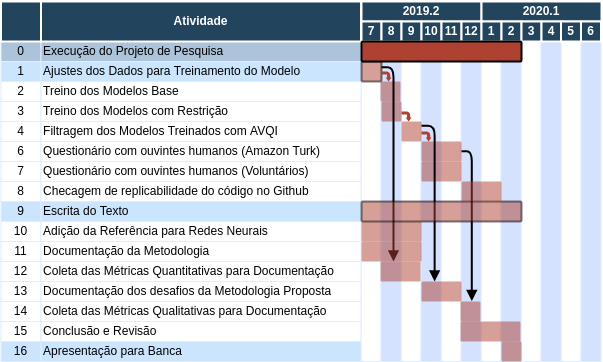
\includegraphics[width=\textwidth]{figuras/cronograma.png}
	\caption{Proposta de Cronograma para Execução do Projeto de Pesquisa}
	\label{fig:processo_de_fala}
\end{figure}

% 

% Com essas proporções para os três conjuntos de dados listados pretendemos concluir  quanto a variabilidade mínima necessária de um mesmo falante e também como o comprimento do conjunto em média afeta a naturalidade final sintetizada.


% \subsection{Proposta de Sentenças 2}
% As referências originais se usam das frases de Harvard extraídas do apêndice do: IEEE Subcommittee on Subjective Measurements IEEE Recommended Practices for Speech Quality Measurements de 1969\footnote{http://www.cs.columbia.edu/~hgs/audio/harvard.html}. Entretanto essas sentenças foram pensadas de maneira anglocêntrica e podem não ser adequadas ao português. Seguindo a literatura de fonoaudiologia recomenda-se usar as frases do CAPE-V para detecção de problemas de fala \footnote{https://www.pucsp.br/laborvox/dicas\_pesquisa/downloads/CAPEV.pdf}  \footnote{https://www.asha.org/uploadedFiles/members/divs/D3CAPEVprocedures.pdf} \footnote{http://www.scielo.br/scielo.php?script=sci\_arttext\&pid=S2317-17822019000100303\&lng=en\&nrm=iso\&tlng=en} totalizando assim 6 frases. Podemos então avaliar a síntese através da análise AVQI 03.01 proposta na literatura de fonoaudiologia para detecção de desvios e vícios de fala\footnote{https://journals.sagepub.com/doi/abs/10.1177/0003489416636131?journalCode=aora}. Esse método se utiliza do Software Praat que é vastamente utilizado no campo de fala para detecção de parâmetros técnicos, como os necessários para equação conforme podemos ver abaixo

% \begin{equation}
% 	\begin{split}
%     	AVQI_{03.01}& = (4.152 - 0.177*CPPs - (0.006*HNR) - (0.037*Shim)\\ 
%     	&+ (0.941*ShdB) + 0.01*Slope + (0.093*Tilt))*2.8902
% 	\end{split}
% \end{equation}

% Para consolidar então os resultados obtidos do AVQI podemos executar uma pesquisa buscando obter o MOS dessas 30 sínteses (6 frases * 5 modelos). Com os resultados desse questionário podemos validar a correlação do MOS com o AVQI e correlacionar o volume de dados disponível a nota do AVQI e ao valor atribuído de média de MOS de Naturalidade com seus respectivos níveis de significância.

  \bibliographystyle{alpha-ime}
  \bibliography{bibliografia}
\end{document}